\documentclass[oneside]{book}
% % % % % % % % % % % % % % % % % % % 
%
%  USEPACKAGES; kept minimal, these can be ammended but not removed.
%
% % % % % % % % % % % % % % % % % % %
\usepackage{fancyhdr}
\usepackage{pdfpages}
\usepackage{graphicx}
%\usepackage{hyperref}
\usepackage[utf8]{inputenc}
\usepackage[colorlinks=true, linkcolor=blue, urlcolor=blue, citecolor=blue, pdfborder={0 0 0}]{hyperref} % removes blue/red boxes on links
\usepackage{longtable}
\usepackage{listings}
\usepackage[acronym]{glossaries}
\usepackage{multirow}
\usepackage{amsmath}
\usepackage{enumitem}
\usepackage{chapterbib}
\usepackage{lipsum} % For sample text

%
% Add other packages here
%

% % % % % % % % % % % % % % % % % % %
% 
% DEFINITIONS FILE
% Change Values of commands in file: "definitions.tex"
%
% % % % % % % % % % % % % % % % % % %
% ADD YOUR NAME HERE
\newcommand{\authorStudentName}{A. N. Onymous}

% REPLACE WITH YOUR STUDENT ID HERE
\newcommand{\authorStudentNum}{M00123456}

% ADD YOUR SUPERVISOR NAME HERE
\newcommand{\supervisorName}{Supervisor NAME}

% CHANGE AS APPROPRIATE
% \newcommand{\documentType}{proposal }
% \newcommand{\documentType}{thesis }
\newcommand{\documentType}{INSERT\_DOCTYPE\_HERE }


\newcommand{\authorName}{Student Name: }
\newcommand{\studentNum}{Student Number: }
\newcommand{\supervisor}{Supervisor: }

\newcommand{\module}{CST\_\_\_\_ - UG/PG Individual Project}

\newcommand{\thesisTitle}{Title of Your Thesis}
\newcommand{\thesisSubTitle}{Sub-Title (if any)}

\newcommand{\degree}{Bachelor OR Master of Science}
\newcommand{\degreeTitle}{DEGREE\_TITLE}
\newcommand{\moduleCoordinator}{Module Coordinator: FULL\_NAME}
\newcommand{\moduleLeader}{Module Leader: Dr FULL\_NAME}

\newcommand{\deptName}{School of Science \& Technology}
\newcommand{\uniName}{Middlesex University}
\newcommand{\campus}{Mauritius}



% % % % % % % % % % % % % % % % % % %
%
% needed for glossary
% comment out as appropriate
% optional
%
% % % % % % % % % % % % % % % % % % %
\makeglossaries

%% GLOSSARY
%makeglossaries 
%% note in alphabetical order - KEEP IT THAT WAY!!!
% \newacronym{}{}{}
\makeglossaries
\newacronym{abac}{ABAC}{Attribute-based Access Control}
\newacronym{acl}{ACL}{Access Control Language}
\newacronym{cqc}{CQC}{Care Quality Commision}
\newacronym{ca1}{CA}{Consensus Algorithms}
\newacronym{ca2}{CAcct}{Contract Account}
\newacronym{cei}{CEI}{Checks, Effects and Interactions}
\newacronym{csrc}{CSRC}{Computer Security Resource Center}
%DDD
\newacronym{dos1}{DOS}{Disk Operating System}
\newacronym{dos2}{DoS}{Denial of Service}
\newacronym{ddos}{DDoS}{Distributed Denial of Service}
%EEE
\newacronym{ecma}{ECMA}{European Computer Manufacturers Association}
\newacronym{eip}{EIP}{Ethereum Improvement Proposal}
\newacronym{eoa}{EOA}{Externally Owned Account}
\newacronym{erc}{ERC}{Ethereum Request for Change}
\newacronym{eth}{ETH}{Ethereum, also denoted $\Xi$}
\newacronym{evm}{EVM}{Ethereum Virtual Machine}
%FF
\newacronym{fat}{FAT}{File Allocation Table}
%GG
\newacronym{gb}{Gb}{Gigabyte}
\newacronym{gpl}{GPL}{General Public License}
%II
\newacronym{ide}{IDE}{Integrated Development Environment}
\newacronym{ierc}{IERC}{Interface for ERC}
\newacronym{iot}{IoT}{Internet of Things}
\newacronym{ibft}{IBFT}{Istanbul Byzantine Fault Tolerant}
%JJ
\newacronym{jit}{JIT}{Just in Time}
\newacronym{lc}{L/C}{Letter of Credit}
\newacronym{lts}{LTS}{Long Term Support}
%MM
\newacronym{mac1}{MAC}{Mandatory Access Control}
\newacronym{md5}{MD5}{Message Digest 5}
\newacronym{mit}{MIT}{Massachusetts Institute of Technology}
%NN
\newacronym{ntfs}{NTFS}{New Technology File Syste}
\newacronym{nist}{NIST}{National Institute of Standards and Technology}
\newacronym{nvm}{NVM}{Non-volatile memory}
\newacronym{nvme}{NVMe}{Non-volatile memory express}
%OOO
\newacronym{oog}{OoG}{Out of Gas}
\newacronym{oop}{OOP}{Object-Oriented Programming}
%PP
\newacronym{p2p}{P2P}{Peer-to-peer}
\newacronym{poet}{PoET}{Proof of Elapsed-Time}
\newacronym{pow}{PoW}{Proof of Work}
\newacronym{pos}{PoS}{Proof of Stake}
\newacronym{qaa}{QAA}{Quality Assurance Agency}
\newacronym{rbac}{RBAC}{Role-based Access Control}
\newacronym{rtw}{RTW}{Return to Work}
%SSS
\newacronym{sc}{SC}{Smart Contract}
\newacronym{sha}{SHA}{Secure Hashing Algorithm}
\newacronym{sop}{SOP}{Standard Operating Procedure}
\newacronym{spdx}{SPDX}{Software Package Data Exchange}
\newacronym{ssd}{SSD}{Solid State Drive}
\newacronym{str}{STRIDE}{Spoofing, Tampering, Repudiation, Information Disclosure, Denial of Service, Elevation of Privileges}
\newacronym{tx}{TX}{Transaction}
%UUU
\newacronym{ucd}{UCD}{Use Case Diagram}
\newacronym{uml}{UML}{Unified Modelling Language}
\newacronym{vm}{VM}{Virtual Machine}
\newacronym{vpn}{VPN}{Virtual Private Network}
\newacronym{wei}{Wei}{1 ETH $\equiv 10^{18}$ Wei}





\begin{document}
\frontmatter
% % % % % % % % % % % % % % % % % % %
% 
%	TITLEPAGE 
%	DO NOT CHANGE
%	MANDATORY
%
% % % % % % % % % % % % % % % % % % %
\begin{titlepage}
    \begin{center}
        
\includegraphics[scale=1.3]{frontmatter/MDX_MRU_LOGO.jpg} \\
        {\huge \module\\}	
        \vspace{2em}

	{\huge \textbf{\thesisTitle \\}}
	{\large \thesisSubTitle\\}	
	\vfill
	
        \authorName \textbf{\authorStudentName} \\
        \studentNum \textbf{\authorStudentNum}\\
        \supervisor \supervisorName \\
        \vfill
        
 	\moduleCoordinator \\
  	\moduleLeader \\
        \vspace{1em}
	\deptName \\
	\uniName \\
	\campus
	\vfill
    % update the command based on the report.. i.e., EITHER \proposal OR \thesis
	This \documentType is submitted for the degree of \\
	\degree \\
	\degreeTitle \\
 	\vfill
	Submission Date: \today 

    \end{center}

\end{titlepage}
\newpage

% % % % % % % % % % % % % % %
%
%	DECLARATION PAGE - 
%	DO NOT EDIT
%	MANDATORY
%   INCLUDE ONLY IN FINAL REPORT!!!
%	File: frontmatter/declarations.tex
%
% % % % % % % % % % % % % % %
\chapter*{Declaration}
	\noindent I, \authorStudentName, declare that this thesis titled, ``\thesisTitle" and the work presented in it are my own. I confirm that:

\begin{itemize} 
\item This work was done wholly for a degree at Middlesex University.
\item Where any part of this thesis has previously been submitted for a degree or any other qualification at Middlesex University or any other institution, this has been clearly stated.
\item Where I have consulted the published work of others, this is always clearly attributed.
\item Where I have quoted from the work of others, the source is always given. With the exception of such quotations, this thesis is entirely my own work.
\item \textit{Any use of GenAI tools has been appropriately acknowledged in this thesis, including the tools used, the purpose of their use, and the extent to which their outputs contributed to the work.}
\item \textit{I remain solely responsible for the content, accuracy, interpretation, analysis, conclusions, and academic integrity of this thesis. Any outputs generated by GenAI tools were critically evaluated, verified, and adapted by me before inclusion.}
\item I have acknowledged all main sources of help\textit{, including any approved use of GenAI tools}.
\item Where the thesis is based on work done by myself jointly with others, I have made clear exactly what was done by others and what I have contributed myself.\\
\end{itemize}

\vspace{0.5cm}

\noindent Signed:\\
\rule[0.5em]{25em}{0.5pt} % This prints a line for the signature

\vspace{1cm}

\noindent Date:\\
\rule[0.5em]{25em}{0.5pt} % This prints a line to write the date
\

	%adds the declaration to the table of contents
	\addcontentsline{toc}{section}{Declaration}
	\newpage

% % % % % % % % % % % % % % %
%
%	ABSTRACT
%	EDIT
%	MANDATORY
%   INCLUDE ONLY IN FINAL REPORT!!!
%	File: frontmatter/abstract.tex
%	
% % % % % % % % % % % % % % %

% AN OPTIONAL PART OF THE REPORT. REMOVE IF YOU DO NOT HAVE AN ABSTRACT
\chapter*{Abstract}
	The Abstract is written here for the FINAL REPORT\\
Approximately $\frac{3}{4}$ to 1 page summary of the whole project from start to finish.
Include a description of:
\begin{itemize}
    \item the area being addressed
    \item what did the research say?
    \item the problem identified \& to be solved
    \item how the problem was addressed (Your Solution / Research)
    \item how the project was evaluated and what conclusions could be drawn from the work. (include key stats/figures from evaluation)
\end{itemize}

You should work on the abstract last as this is the summary of what was achieved throughout the project. i.e., key information from all chapters provided as a summary.
	%adds the abstract to the table of contents
	\addcontentsline{toc}{section}{Abstract}

% % % % % % % % % % % % % % % %
%
%	AKNOWLEDGEMENTS
%	EDIT
%	OPTIONAL
%	File: frontmatter/acknowledgements.tex 
%
% % % % % % % % % % % % % % % %
\chapter*{Acknowledgements}
	The acknowledgements section goes for recognising any work that had a big impact / was useful in building yours (e.g., can be libraries, frameworks, repositories, research work) and also Thanks to those who supported or contributed to the work! e.g., Parents, siblings, friends, supervisor\ldots
	%adds acknowledgements to the table of contents
	\addcontentsline{toc}{section}{Acknowledgements}
	\newpage
	
% % % % % % % % % % % % % % % %
%
%	TABLE OF CONTENTS
%	DO NOT EDIT	
%	AUTOMATICALLY GENERATED
%	MANDATORY	
%
% % % % % % % % % % % % % % % %
\tableofcontents

% % % % % % % % % % % % % % % %
%
%	LIST OF FIGURES 
%	EDIT AS APPROPRIATE
%	AUTOMATICALLY GENERATED
%	OPTIONAL	
%
% % % % % % % % % % % % % % % %
\listoffigures

% % % % % % % % % % % % % % % %
%
%	LIST OF TABLES 
%	EDIT AS APPROPRIATE
%	AUTOMATICALLY GENERATED
%	OPTIONAL	
%
% % % % % % % % % % % % % % % %
\listoftables


% % % % % % % % % % % % % % % %
%
%	GLOSSARY 
%	EDIT AS APPROPRIATE
%	AUTOMATICALLY GENERATED
%	OPTIONAL	
%	requires lines 38-39 uncommented
%
% % % % % % % % % % % % % % % %
\printglossary[title=Acronyms, type=\acronymtype]
\printglossary



\mainmatter
% % % % % % % % % % % % % % % % % %
%
%	HEADERS & FOOTERS
%	DO NOT EDIT
%	MANDATORY
%
% % % % % % % % % % % % % % % % % % %
\pagestyle{fancy}
\rhead{\leftmark}
\lhead{\empty}
\lfoot{\empty}
\cfoot{\thepage}
\rfoot{\empty}

% \pagestyle{fancy}
% \fancyhf{} % Clear all header and footer fields
% % Update the left header with the chapter title using \leftmark
% \fancyhead[R]{Chapter \thechapter: \leftmark}
% \renewcommand{\chaptermark}[1]{\markboth{#1}{}}


% % % % % % % % % % % % % % % %
%
% 	CONTENT
% 	EDIT
% % % % % % % % % % % % % % % %
\chapter{Introduction}
% THE PROPOSAL STRUCTURE \\
% This chapter should provide overview of the project, while also providing a sensible timeline for the different tasks involved. Explain the aims, objectives, problem statement, rationale, and methodology to be employed. Note: that you need to include in-text citations throughout the whole report!! Sources should be mainly from Conference Proceedings or Journal Publications. You can search for scholarly articles/literature on search engines like \href{https://scholar.google.com/}{Google Scholar}. Other sources like: IEEEXplore, ScienceDirect, ACM, Springer, Elsevier, etc\ldots
% \vfill
% Overall, structure for the \textbf{Proposal Document} and Introduction Chapter should be something as follows:
% \begin{enumerate}[label=(\alph*)]
% \item Background of Study
% \item Problem Statement
%     \begin{enumerate}[label=(\roman*)]
%       \item Existing Solutions / Works / Research
%     \end{enumerate}
% \item Description of System
%     \begin{enumerate}[label=(\roman*)]
%       \item Aims
%       \item Objectives
%     \end{enumerate}
% \item Key Activities of Project
%     \begin{enumerate}[label=(\roman*)]
%       \item Software Development OR Research Methodology
%       \item Project Deliverables
%     \end{enumerate}
% \item Project Plan
%     \begin{enumerate}[label=(\roman*)]
%       \item Milestones
%       \item Gantt Chart
%     \end{enumerate}
% \item Resources Required
%     \begin{enumerate}[label=(\roman*)]
%       \item Development Languages/Tools OR Research Tools
%       \item Possible Hardware/Technologies/Frameworks
%     \end{enumerate}
% \item References / Bibliography
% \end{enumerate}
This chapter should provide an overview of the project, what is the setup, what is the problem, what is the scope and finally the contribution/solution.\\
A small breakdown and description of these sections:

\section{Background of Study}
brief history of technologies and products/suites that exist currently in your field of study. provide an overall background on what is being done right now (e.g., with similar apps or projects or research) in this field.. \\
Do they have limitations? if so what are they.. can also give reasons on why it is like it is.. (e.g., technology is limited, implementation wasn't well carried out, there is too much to cater for) \\
what is the issue (briefly)? \\
what issues you’re planning to address (briefly)?

\section{Problem Statement}
A small intro into the problem. specify in details the impact the problem causes (all relevant to your project title and validating the development of your project) and briefly how your project will help address that issue

\subsection{Existing Solutions / Works / Research \textit{(do not include in FINAL REPORT [already covered in Chapter 2])}}
talk about existing research, projects and commercial apps that already exist (relevant to your study), and discuss what’s lacking, identify problems and gaps that they haven't addressed yet, which you can improve through your application. \\
A quick comparison table will also be good.
Can be disregarded for Chapter 1 if you have a full fledged Literature Review Chapter.


\section{Description of System OR Research Scope}
give your idea of what the ideal solution should be like if development is involved. If research then discuss what is the scope of this project.

\subsection{Aims}
The overall milestones of the project, and what the project should have achieved at the end. Should be 1 small paragraph and around 2 to 5 sentences.

\subsection{Objectives}
smaller tasks of how you will achieve those aims, in bullet form.
brief overview: e.g.,:
\begin{itemize}
    \item The initial project proposal,
    \item Detailed Research / Literature Review,
    \item Gather System Requirements (including Functional/Non-Functional Requirements, and other system diagrams like UML, wireframes, project technology architecture diagram), OR Research Methodology and Scope in depth - describing any use of a theoretical framework to conduct/carry the whole research work,
    \item Developing, Testing, and Documentation of the Solution, OR Overall Research work itself i.e., collection of data (research papers etc), the analysis, comparison, drawing knowledge out of the analysis done,
    \item Evaluation of the project/solution OR Research work, and
    \item Deliver the Final Thesis Report with documentation along with VIVA Presentation.
\end{itemize}

\subsection{Research Questions}
Keep in mind that the Research Workflow for any thesis is typically: Aims \& Objectives → Problem Statement → Gaps from LR → Research Questions\\
Each stage feeds forward into the next.\\
Research Questions must directly address:
\begin{itemize}
    \item The Objectives,
    \item The Problem, and
    \item The Gaps identified in the Literature Review.
\end{itemize}

\section{Key Activities of Project}
\subsection{Software Development OR Research Methodology}
which methodology you will use to implement or conduct the analysis?  \\
Development wise there are: waterfall, agile, scrum, prototyping, RAD, etc\ldots \\
Research design wise we have: quantitative, qualitative, mixed-methods. Research Methodology you need to describe\ldots\\
Only include this section in UG projects for CW1 - remove it from the FINAL REPORT.\\

\subsection{Project Deliverables}
what will be the deliverables of your project? \\
(Literature Review, Testing Results [e.g., functional, unit, pilot, etc], app/project documentation, a prototype of the app/project, OR Research Output, Analysis, Results, Evaluation, data, \& discussions, etc\ldots)

\section{Project Plan}
\subsection{Milestones}
Here you could just list the main tasks. They usually stem from the Objectives, Project Deliverables, and other important tasks of the project.
\subsection{Gantt Chart}
this section will be mainly the Gantt chart, but you can add a bit more info through a paragraph about each task.

\section{Resources Required}
\subsection{Development Languages/Tools OR Research Tools}
Describe any tools you may be using for the project be it development or research. e.g., Kotlin, Dart, Android Studio, Visual Studio, etc.
\subsection{Possible Hardware/Technologies/Frameworks}
Any technologies you think that will be useful for the project. e.g., APIs, Cloud services, SDKs, etc\ldots

\section{Key Contributions \textit{(only in for FINAL REPORT)}}
Add this section in the final report\ldots \\
Highlight the original contributions your thesis makes to the field.

\section{Summary of Chapters \textit{(only in for FINAL REPORT)}}
Add this section in the final report\ldots \\
Summarise each chapter after chapter 2 featuring in the final report, with 1 paragrpah of about 3 to 5 lines per chapter.

\chapter{Literature Review}
Each project has its own unique flow, would recommend you write a sample flow (like a quick table of contents with sections \& sub-sections) of the Literature Review chapter and ask for feedback from your supervisor and implement it.\\
But general idea:\\
\begin{itemize}
    \item Purpose?? It is to provide a comprehensive and critical overview of existing literature on a topic.\\
    \item How?? By summarising , evaluating, and synthesising the relevant research and articles.\\
    \item Why?? To identify gaps, trends, contradictions, and key findings. BUT also to justify your methods.
\end{itemize}


To start off the section you can provide a small intro and summary on what the section discusses\ldots

\section{Introduction}
Introduce the purpose and scope of the literature review.

\section{Background of "YOUR topic"}
Provide a comprehensive background on the chosen topic (e.g., blockchain, AI).
Explain the evolution and context of the topic.

\section{Problem Description}
Elaborate on the specific problem identified in the introduction.

\section{Sources \& Impacts}
Explore relevant sources and literature related to the problem.
Discuss the impact of the problem on the field or industry.

\section{Existing Research / Solutions}
Review existing research and solutions addressing the identified problem.
Identify strengths and weaknesses of current approaches.

\section{Comparative Analysis}
Compare different projects, algorithms, solutions, or research work to your project title. Think about using a framework to better structure the comparison.

\section{Critical Analysis}
Analyse the strengths and limitations of existing research/projects/solutions critically.

\section{Summary of Findings}
Summarise the key findings from the literature review.

\section{Proposed Solution}
Introduce the proposed solution or approach based on the literature reviewed and gaps identified.


\chapter{Analysis \& Design $\mid$ Research Methodology}
This chapter as well is a little flexible, since each project will have its own flow and sections.
Again, implement the feedback provided by your supervisor \\

Development based Project Structure:
\begin{itemize}
    \item Development Methodology \\
Specify the methodology chosen for the development process, with justification.

    \item Functional and Non-Functional Requirements \\
Define the functional and non-functional requirements of the proposed solution.

    \item UML Diagrams \\
Present UML diagrams, including Use Case, Activity, Sequence, and Class diagrams (some or most of these diagrams wont be applicable for you).

    \item Other Diagrams
    \item Database Design \\
Provide a database diagram outlining the structure of the database.

    \item Architecture Diagram \\
Illustrate the overall architecture of the proposed system.

    \item Wireframes and UI Designs \\
Provide some wireframes and designs of the proposed system.

    \item Initial Development \& Progress \textit{(only in UG projects for CW1)} \\
Provide description, screenshots, diagrams, and other relevant materials in relation to the development you have been able to do until this stage.

    \item Evaluation Plan \textit{(only in UG projects for CW1)} \\
Give a description on what the finalised version of evaluation looks like. If you plan to recruit participants for this step, link it to the Ethics approval application proof. Otherwise, describe the methodology, taxonomy or framework you will be using to evaluate the project.
\end{itemize}

\vspace{2em}


Research based Project Structure:
\begin{itemize}
    \item Research Design \\
What was analysed\\
What is the project trying to solve/find\\
The key search criteria you used to search for papers\\
The main research repositories you got the papers from\\
Discuss why the chosen method was preferred. what you sought to find out.

    \item Research Methodology \\
Describe and justify the methodology you used to perform the analysis

    \item Result Analysis Method \\
Describe in detail the procedure you followed, e.g., surveys, interviews, case studies, experiments, simulation.\\
Enumerate and Describe: what and how did you analyse the data/results

    \item Limitations \textit{(only in UG projects for CW1)} \\
What are the current limitations you have identified that might halt further progress.
    \item Initial Research Outcome \& Progress \textit{(only in for CW1)} \\
Provide an update on what you have been able to do until this stage.
    \item Evaluation Plan \textit{(only in UG projects for CW1)} \\
Give a description on what the finalised version of evaluation looks like. If you plan to recruit participants for this step, link it to the Ethics approval application proof. Otherwise, describe the methodology, taxonomy or framework you will be using to evaluate the project.

    \item Points to consider and include:

    \begin{enumerate}[label=(\alph*)]
        \item Research Approach Selection (Quantitative or Qualitative) (Theoretical or Practical Research)
        \item Optionally can look at a hypothesis
        \item Identification of Variables and Measures
        \item Sample Size and Sampling Methodology (ensure good representation of the population)
        \item Methods of Data Collection (surveys, interviews, observations, experiments, etc)
        \item Analysis Techniques
        \item Ethical Considerations
    \end{enumerate}
        
\end{itemize}


\chapter{Implementation \& Testing $\mid$ Analysis}
Can have small intro to the section and whats next to come. \\
Again, implement the feedback provided by your supervisor. \\

\textbf{For Development projects:}\\
This part of the chapter is mainly about discussing the development journey, the features done (scripts responsible for it), the hurdles/challenges you faced, what was adapted/changed from initial idea, what has been improved, describe what the solution does.
You can consider adding diagrams where it fits. E.g., flowcharts, process or logic flow of system. \\


Development based Project Structure:
\begin{itemize}
    \item Implementation \\
talk specifications, the requirements, describe what the solution does, development environment, show architecture/process/logic diagram of the overall system but development wise, and Overall Project (can consider flowchart too) \\
describe project folder structure \\
talk about the features of dataset (if you have Machine Learning), and describe each. \\
give snippets of code to explain main parts and logic
(you will know how to structure the sub-sections based on the ideas above - consider using tables to better structure/present everything)\\
Sample Structure:
\begin{enumerate}[label=(\alph*)]
        \item Key Features
        \item Project Folder Structure (Description)
        \item Code Explanation (Documentation) \\
Only provide small snippets of the main scripts and explain its use/task
        \item Challenges encountered
    \end{enumerate}

    \item Testing \\
each test performed can be a different section \\
tabulate results, critically analyse them \\
functional testing, unit testing, black box, white box, script based unit tests, etc.. \\
at the end can also state other possible considerations to add \\
Sample Structure:
\begin{enumerate}[label=(\alph*)]
    \item Testing Procedures: Methods and criteria used for testing the validity and reliability of the findings
    \item Functional Testing
    \item Unit Testing
    \item Performance Testing
    \item Black box Testing
    \item Heuristics/HCI (for projects where UI is important)
    \item Any other Framework applied
\end{enumerate}

\end{itemize}

\vspace{2em}

\textbf{For Research projects:}\\
Describes the analysis procedure and how they answer research questions/hypothesis.\\
Note: Can be broken into 2 chapters depending on analysis to be performed – Confirm with your supervisor

Research based Project Structure:
\begin{itemize}
    \item Data Cleaning \& Preparation \\
Clean the data by checking for missing values, inconsistencies, and outliers. \\
Code your categorical variables and prepare your data for analysis using statistical software like SPSS or R.

    \item Analysis Techniques \\
Elaborate on the analysis techniques. Explain why it has been chosen and how it has been used. Ensure that we can replicate the analysis and same results will be obtained.

    \item Result Analysis Method \\
Describe in detail the procedure you followed, e.g., surveys, interviews, case studies, experiments, simulation.\\
Enumerate and Describe: what and how did you analyse the data/results

    \item Limitations \\
What are the current limitations you have identified that might halt further progress.

    \item Points to consider and include:

    \begin{enumerate}[label=(\alph*)]
        \item Research Approach Selection (Quantitative or Qualitative) (Theoretical or Practical Research)
        \item Optionally can look at a hypothesis
        \item Identification of Variables and Measures
        \item Sample Size and Sampling Methodology (ensure good representation of the population)
        \item Methods of Data Collection (surveys, interviews, observations, experiments, etc)
        \item Analysis Techniques
        \item Ethical Considerations
    \end{enumerate}
        
\end{itemize}


\chapter{Evaluation $\mid$ Research Results}
This chapter as well is a little flexible, since each project will have its own flow and sections.
Again, implement the feedback provided by your supervisor \\

Development based Project Structure:
\begin{itemize}
    \item Purpose of “Chosen Methodology(ies)” \\
Discuss why the chosen method was preferred.\\
What had you sought to find out? (Research Questions)

    \item Evaluation Method \\
outline the procedure followed to do the evaluation,\\
any considerations to be made\\
assess the methodology as well (review backed mainly by literature).\\
how does the methodology or experiment answer/leads you to the research questions – \textit{very important to evaluate this as well}.

    \item Results Analysis \\
present and discuss the results – be it positive or negative. (normally in tabular format)\\
possibly also compare them to existing works (to see if it was successful, and to what extent)\\
highlight any key statistic or finding you found


    \item Reflection on the Outcome \\
interpret what was the overall outcome (the bigger scope).\\
Suggestions on steps that could be taken to improve results/outcome.\\
overall discussion on recommendations for improved results. your experience.

\end{itemize}

\vspace{2em}

Research based Project Structure:
\begin{itemize}
    \item Discussion and Interpretation of Findings \\
Analyse everything in detail, point by point. Using key statistics, and relate findings to aims, objectives, problem statement.\\
You would have tables here to describe most of the findings\\
Perform a Comparison of findings with existing literature

    \item Analysis of the Research Questions \\
What had you sought to find out? (Research Questions) \\
List the research questions and explain how they were solved/answered.\\
Do same for your hypothesis. This should be in-depth.

    \item Summary of Findings \& Key Contributions \\
Interpret what was the outcome. what could be done to improve results. other suggestions for improved results. your experience.
        
\end{itemize}


\chapter{Conclusion \& Future Work}
Provide a summary of the project findings and any other relevant information.  What did you learn? What was interesting?
\section{Project Analysis}
Give overall verdict on the project and analyse the journey\\
Concise summary of the research findings.\\
Final thoughts and conclusions drawn from the research.

\section{Limitations of Project}

\section{Future Works}
Suggestions for future research and possible avenues\\
What other points/techniques could be considered if had more time \cite{seyyar2020privacy}.



% % % % % % % % % % % % % % % %
%
% 	BIBLIOGRAPHY 
%	MANDATORY 
% 	Use basic BiBTex options, IEEE-like numbered references
% 	file: references.tex
%
% % % % % % % % % % % % % % % %
\bibliographystyle{plain}
\addcontentsline{toc}{chapter}{Bibliography}
\bibliography{references}


% % % % % % % % % % % % % % % %
%
% 	Sample Structure for your VIVA Slides. Adapt from the structure
%   Remove this section when writing the report
%
% % % % % % % % % % % % % % % %
\chapter*{VIVA Slides Structure}
    \begin{enumerate}
        \item Cover Slide \\
        Include your Name, Student number and Project title.
        \item Background \\
        Present a short overview of the topic being studied and undertaken as part of the project.
        \item Problem Description \\
        Address clearly the problem that you are intending to solve.
        \item Existing Solutions/Research \\
        Here you can give a comparative table like in Chapter 2 Literature Review, Or compare and discuss other existing products/solutions you investigated.
        \item Proposed Solution/Analysis Conducted \\
            Development based Project Structure (\textit{Proposed Solution}):
                \begin{itemize}
                    \item Present all the features of your proposed artefact. Add screenshots as well. Specify how it is going to solve the problem that you have identified and how (again linked to the Problem Statement and Aims/Objectives).
                \end{itemize}
        
        Research based Project Structure (\textit{Analysis Conducted}):
                \begin{itemize}
                    \item Discuss the Research Methodology, method chosen for Analysis and the outcome of the Analysis. Provide the Limitations around the end. You should justify why the chosen method..\\
                    \item Finally, the discussion should be about the findings of the analysis and how it helps solve the Research Questions.
                \end{itemize}
        \item Evaluation/Results \\
        How you evaluated your proposed solution / OR results given. Present the results (including key stats if any).
        \item Conclusion \\
        You can include a brief concluding slide at the end.
        \item References \\
        List of all references used in the slides.

    \end{enumerate}


% % % % % % % % % % % % % % % %
%
% 	Appnendix		
%	OPTIONAL	
% 	file: appendix/meetings.pdf 
%   Include any additional supporting content which might break the flow of the report
%   Any additional data, graphs, questionnaire, Ethics approval or Ethics Screening Form, User Guide/Manual
%   Try to structure it logically
%
% % % % % % % % % % % % % % % %
\appendix
\part*{Appendices}
\addcontentsline{toc}{part}{Appendices}

\chapter{Tutorials}

\begin{figure}
	\centering
	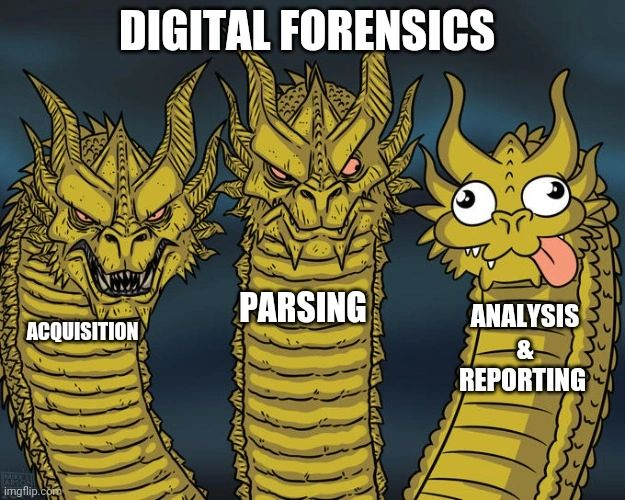
\includegraphics[scale=0.35]{appendix/images/digitalForensics.jpg}
	\caption{Test caption number}
\end{figure}

\section{LaTeX TUTORIALS}
\subsubsection{Citation \& Reference}
tutorial for referencing: This is a sample text \cite{daghmehchi2022memory} 

Exercises show two there are two parts to a citation: the citation; and the reference. There are many styles and configurations of the citations and references, which the exercises will make clear. 

Essentially, to start with, we are going to keep this simple and use the plain bibliography setting. As we advance the national bibliography package can be used and this is in the exercises on citations. This setting orders all bibliography items in alphabetical order and only uses the cite command. It does have its restrictions and we will come across these and how to cope with them. The following is an example paragraph using citations and a plain bibliography and should be adequate to get us started.


The first generation of Neural Networks are generally considered as Perceptrons \cite{rosenblatt1958perceptron}. Minsky and Papert \cite{minsky1969perceptrons} wrote a critique of the perceptron which showed that it could not solve non-linear problems, typically XOR. To solve the non-linear problem Rumelhart, Hinton and Williams \cite{rumelhart1985learning} made an enormous contribution with the Back-propagation error Artificial Neural Network, ANN. This and related ANN are generally referred to as second generation and inspire many of the techniques used in machine learning. The third generation of neural networks are based on biologically-inspired neurons and are generally referred to as, ``spiking neurons''.  Oddly many third generations are based on research pre-dating to first and second generations, namely Hebbian Learning \cite{Hebb}. These spiking neurons can be built into bigger networks to solve complex problems, e.g., see \cite{huyck2013compensatory}.

\subsubsection{Example of glossary}
There are several blockchain \gls{ca1} but three of interest are: \gls{poet}, \gls{pow} and \gls{pos}.

\gls{poet} is fast and can only be used on permission blockchains. \gls{pow} is computationally expensive and can be used on permissionless blockchains, many researchers have commented that \gls{pow} is unsustainable. \gls{pos} is less computationally expensive and can be used on permissionless blockchain technology. 

\subsubsection{Schedule}
You can reference the image as follows: Fig.\ref{fi:LinuxDir}.

% % % % % % % % % % % % % % %
%
%	INCLUDING FILES	
%	File: appendix/images/linux-directory-structure.png
%	N.B. 	This is compiled from the parent directory.
%		Hence referencing appendix/images directory from within appendix/images
% 
% % % % % % % % % % % % % % %
\begin{figure}
\centering
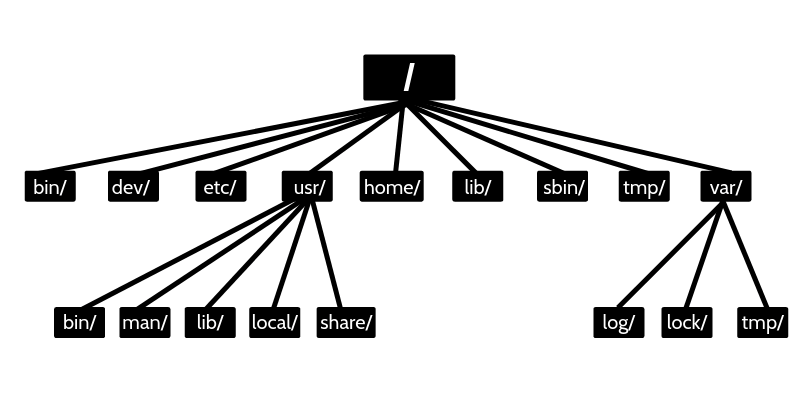
\includegraphics[scale=0.4]{appendix/images/linux-directory-structure.png}
\caption{Linux Directory Structure}\label{fi:LinuxDir}
\end{figure}


\begin{figure}
	\centering
	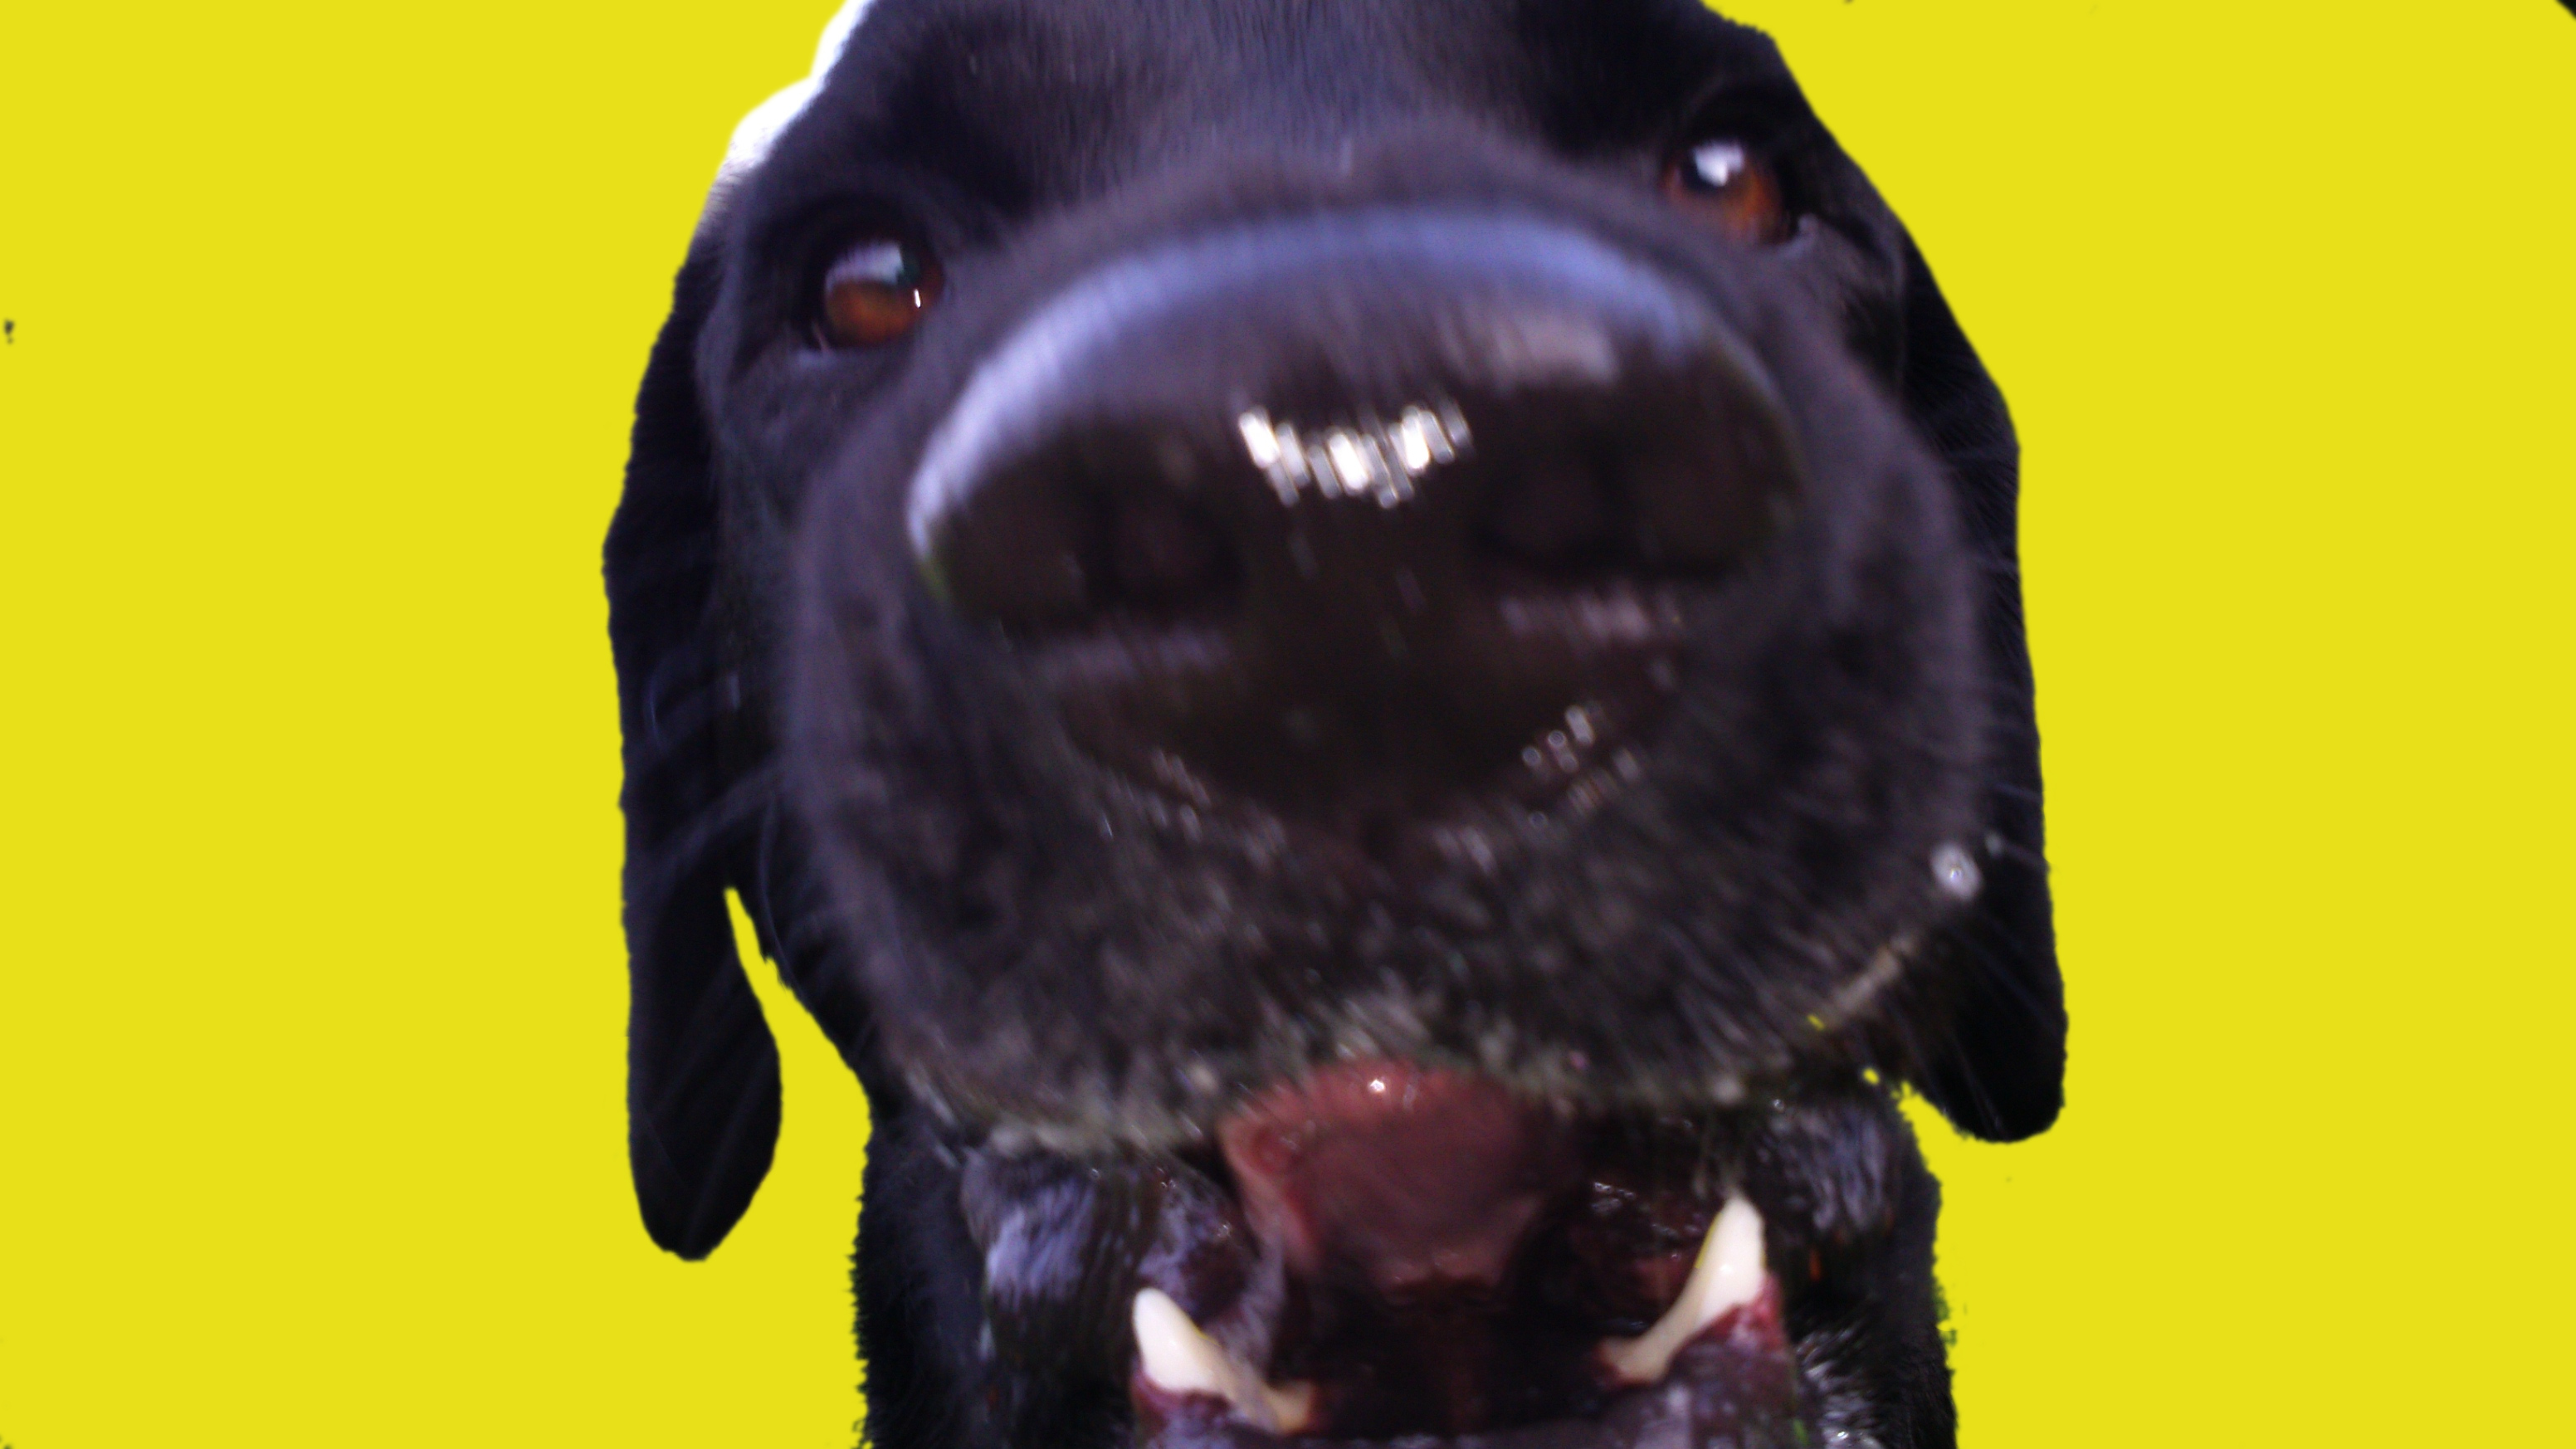
\includegraphics[scale=0.1]{appendix/images/awo}
	\caption{Test caption number}
\end{figure}

\newpage

\subsubsection{Experiment 1}
Use graphics to display results. Most results can be shown in tables. Use package longtables if you have trouble getting all data into a single page. Remember to label and reference the table.

\begin{table}
	\centering
	\begin{tabular}{|c|l|l|l||r|}\hline
	Run	&	x	&	y 	&	z	& Time/ms\\ \hline
	1	&	100	&	2.5	& 	1.06	& 60000 \\ \hline
	2	&	200	&	4.5	&	1.45	& 50000 \\ \hline
	3	&	500	&	5.5	&	1.5	& 40000 \\ \hline
	\end{tabular}
	\caption{Experiment 1 Results}
	\label{ta:ex1}
\end{table}


\subsubsection{Experiment 2}
Experiment 2 should differ from Experiment 1. Each experiment should be repeated a number of times for reproducibility. Do not confuse Experiment 2 as a repeat of Experiment 1, they are different. 

\begin{table}
	\centering
	\begin{tabular}{|c|l|l|l||r|}\hline
	Run	&	x	&	y 	&	z	& Time/ms\\ \hline
	1	&	100	&	2.5	& 	1.06	& 60000 \\ \hline
	2	&	200	&	4.5	&	1.45	& 50000 \\ \hline
	3	&	500	&	5.5	&	1.5	& 40000 \\ \hline
	\end{tabular}
	\caption{Experiment 2 Results}
	\label{ta:ex2}
\end{table}


\chapter{Ethical Approval}
The below form needs to be filled first, then signed by your supervisor.
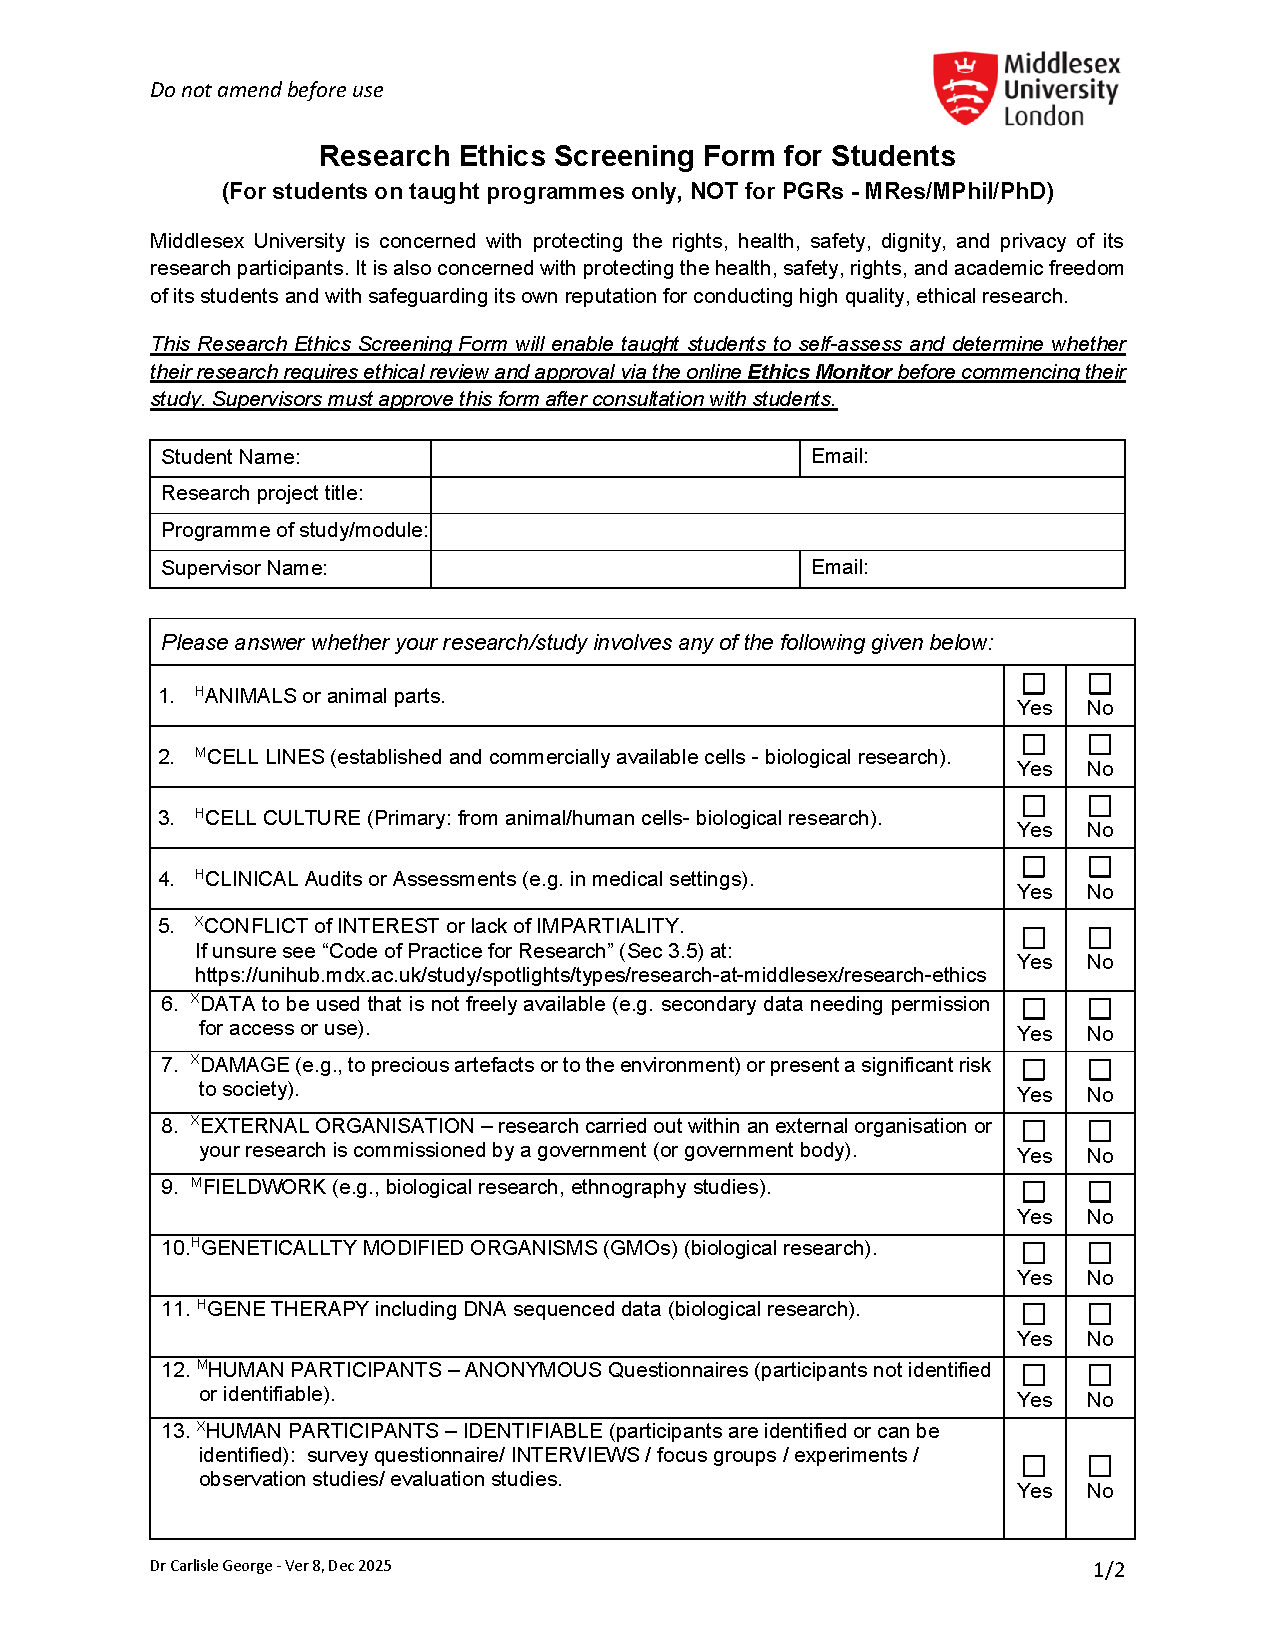
\includepdf[pages=-, scale=0.75]{appendix/MUR Research Ethics Screening Form for Students V8.pdf}

\chapter{Meeting Log with Supervisor}
%include pdf file, "meetings.pdf". 
% The options include only page 1, because it is already a4, it is scale down to 0.75. 
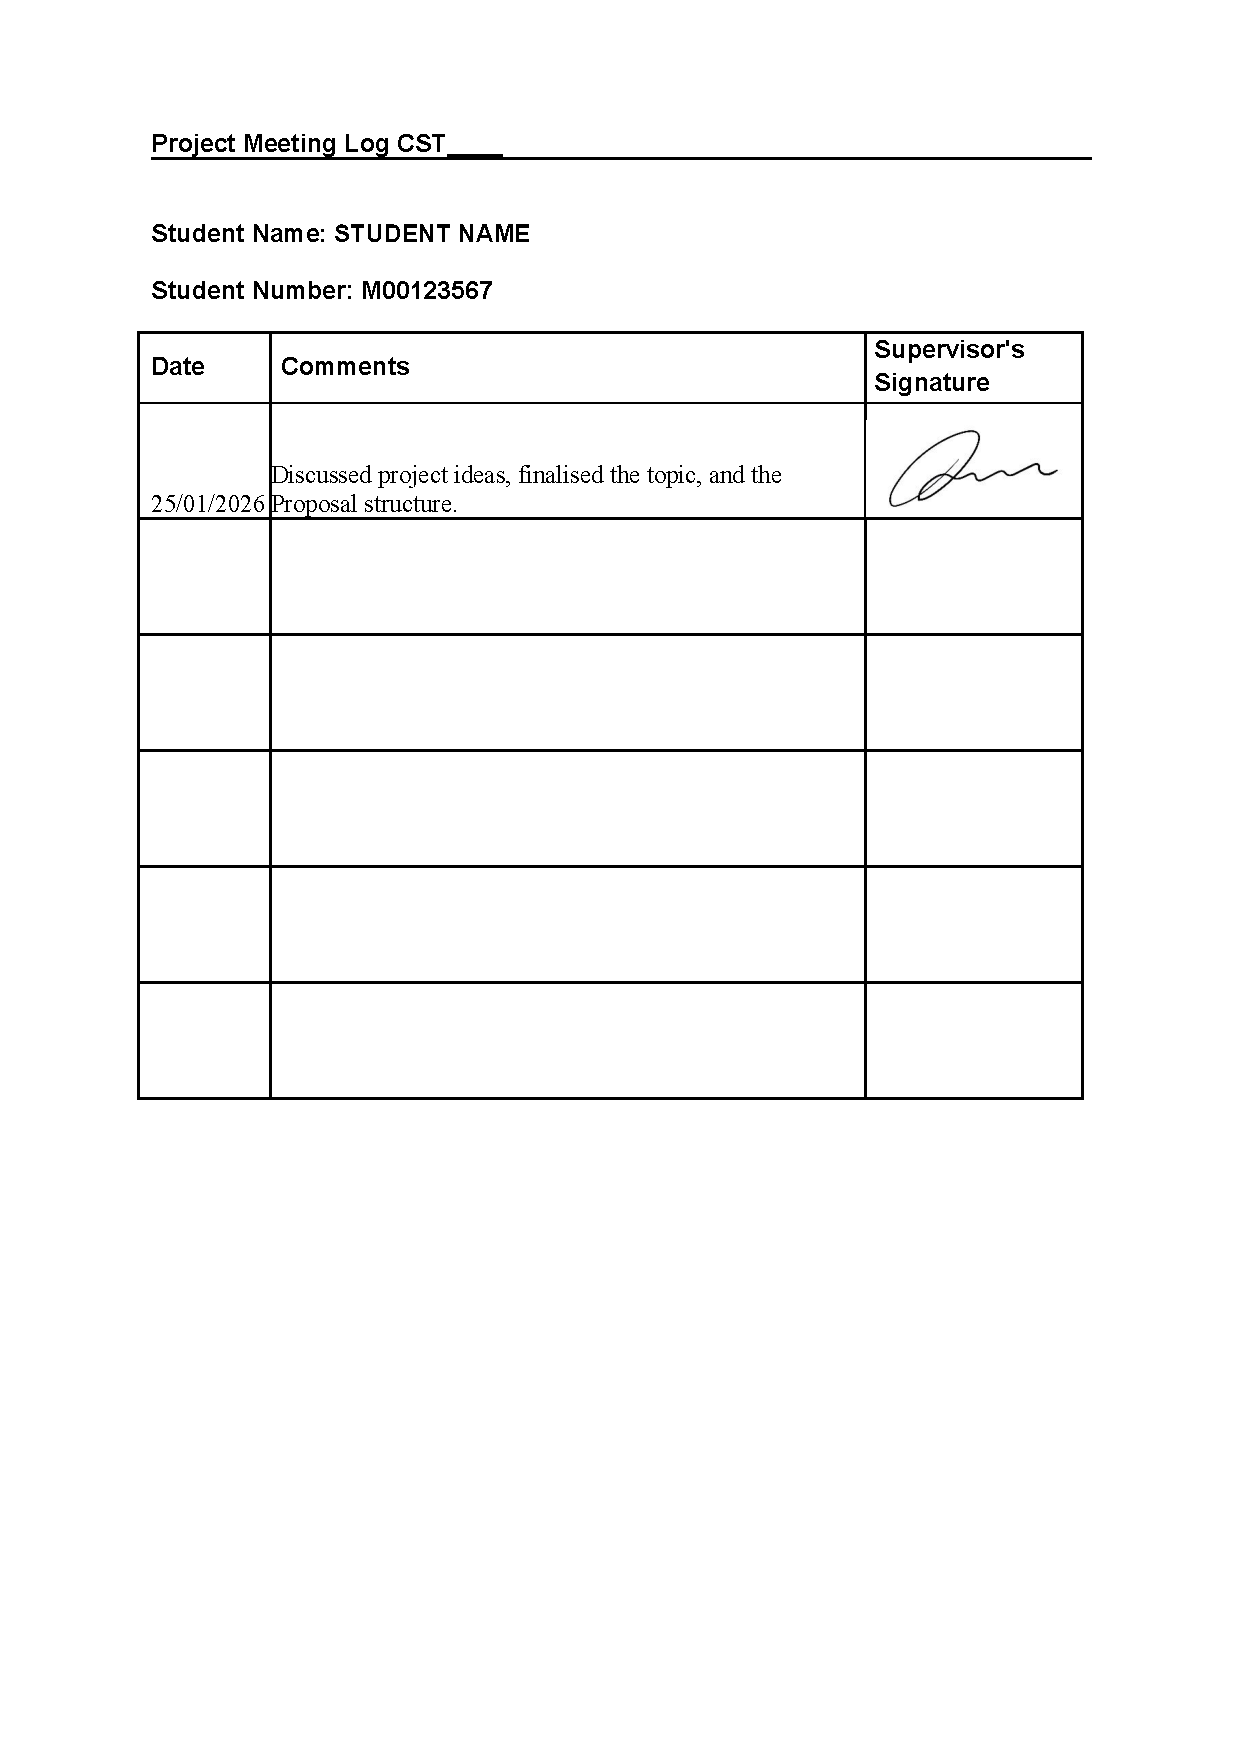
\includepdf[pages=1,scale=0.75]{appendix/Meeting Logs.pdf}

\end{document}
